% ============================================================
%  Hardware Color Plugin — Feature Reference
%  Paste into Overleaf (pdfLaTeX).
% ============================================================
\documentclass[11pt, letterpaper]{article}

\usepackage[margin=1in]{geometry}
\usepackage{amsmath, amssymb}
\usepackage{booktabs}
\usepackage{hyperref}
\usepackage{caption}
\usepackage{float}
\usepackage{xcolor}
\usepackage{tikz}
\usetikzlibrary{shapes.geometric, arrows.meta, positioning, calc}

\title{\textbf{Hardware Color Plugin}\\[4pt]
       \large Controls, Signal Chain, and Analysis Implementation}
\author{John Micensky}
\date{\today}

% ============================================================
\begin{document}
\maketitle
\tableofcontents
\vspace{1em}

% ------------------------------------------------------------
\section{Overview}

The Hardware Color plugin applies a measured analog device's nonlinear
signature to an input audio stream.  It is a stereo VST3/AU that loads
an \emph{artifact file} — a compact JSON bundle produced by the
AnalogColorMeasurement capture tool — and uses the embedded
L-N-L model to colour audio in real time.

Three front-panel controls let the user adjust how aggressively the
device character is imposed: \textbf{Drive}, \textbf{Weight}, and
\textbf{Mix}.

% ------------------------------------------------------------
\section{Signal Chain}

The per-channel processing path, executed in
\texttt{PluginProcessor::processBlock}, is:

\begin{center}
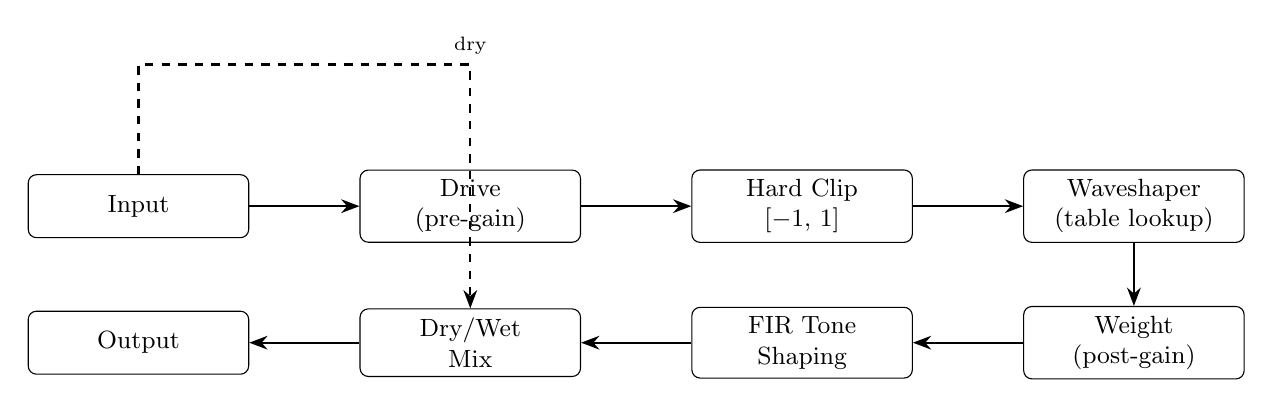
\begin{tikzpicture}[
    node distance = 8mm and 14mm,
    box/.style    = {rectangle, draw, rounded corners=3pt,
                     minimum width=28mm, minimum height=8mm,
                     font=\small, align=center},
    arr/.style    = {-Stealth, thick}
]
  \node[box] (in)    {Input};
  \node[box, right=of in]  (drive)  {Drive\\(pre-gain)};
  \node[box, right=of drive] (clip)  {Hard Clip\\{$[-1,\,1]$}};
  \node[box, right=of clip]  (ws)    {Waveshaper\\(table lookup)};
  \node[box, below=of ws]    (wt)    {Weight\\(post-gain)};
  \node[box, left=of wt]     (fir)   {FIR Tone\\Shaping};
  \node[box, left=of fir]    (mix)   {Dry/Wet\\Mix};
  \node[box, left=of mix]    (out)   {Output};

  \draw[arr] (in)    -- (drive);
  \draw[arr] (drive) -- (clip);
  \draw[arr] (clip)  -- (ws);
  \draw[arr] (ws)    -- (wt);
  \draw[arr] (wt)    -- (fir);
  \draw[arr] (fir)   -- (mix);
  \draw[arr] (mix)   -- (out);

  % dry tap
  \coordinate (tap) at ($(in)!0.5!(drive) + (0,18mm)$);
  \draw[arr, dashed] (in.north) |- (tap) -| (mix.north)
        node[midway, above, font=\scriptsize] {dry};
\end{tikzpicture}
\end{center}

\noindent
The dry signal is captured \emph{before} any processing and blended
back at the Mix stage.

% ------------------------------------------------------------
\section{Controls}

\subsection{Drive}

\begin{description}
  \item[Range] \(0.0 \;\text{--}\; 10.0\) \quad Default: \(1.0\)
  \item[Step]  \(0.01\)
\end{description}

Drive is a simple pre-gain scalar applied to every sample before the
waveshaper:
\[
  x_{\text{in}} = s[n] \times d_{\text{drive}}
\]
The result is hard-clipped to \([-1,\,1]\) before being passed to the
waveshaper lookup.  At the default value of~\(1.0\) the signal enters
the waveshaper at the same amplitude it was captured at, reproducing
the device's measured behaviour exactly.  Values above~\(1.0\) push
more of the waveform into the saturating region of the waveshaper
curve; values below~\(1.0\) keep the signal in the more linear
small-signal regime.

\subsection{Weight}

\begin{description}
  \item[Range] \(0.0 \;\text{--}\; 2.0\) \quad Default: \(1.0\)
  \item[Step]  \(0.01\)
\end{description}

Weight is a post-nonlinearity output scalar:
\[
  s_{\text{ws}}[n] = \textsc{Waveshaper}(x_{\text{in}}) \times w_{\text{weight}}
\]
It controls how loudly the coloured signal emerges from the waveshaper
before FIR tone shaping and wet/dry mixing.  At~\(1.0\) the
waveshaper's own small-signal gain (which has been normalised to unity
during analysis) is preserved.  Raising Weight brightens the overall
level of the wet signal without altering the nonlinear character;
lowering it fades the coloured path while the Mix control's dry path
remains unaffected.

\subsection{Mix}

\begin{description}
  \item[Range] \(0.0 \;\text{--}\; 1.0\) \quad Default: \(1.0\)
\end{description}

Mix is a linear dry/wet blend applied \emph{after} all tone shaping:
\[
  s_{\text{out}}[n] = s_{\text{dry}}[n]\,(1 - m) \;+\; s_{\text{wet}}[n]\, m
\]
where \(s_{\text{dry}}\) is the signal captured before Drive, and
\(s_{\text{wet}}\) is the FIR-shaped, weighted output.  At~\(1.0\)
only the processed signal is heard; at~\(0.0\) the plugin is fully
transparent.  Because the dry tap precedes Drive, Mix behaves as a
true parallel blend regardless of Drive or Weight settings.

% ------------------------------------------------------------
\section{Artifact Loading and Sample-Rate Adaptation}

The plugin loads an artifact file at any time via
\texttt{HardwareColorProcessor::loadArtifact}.  The artifact contains:
\begin{itemize}
  \item \textbf{FIR coefficients} (512 taps) — derived from the
        device's measured frequency response.
  \item \textbf{Waveshaper table} (1024 entries) — mapping input
        amplitude to output amplitude over \([-1,\,+1]\).
  \item \textbf{Stored frequency-response data} — downsampled
        magnitude-vs-frequency pairs used for FIR reconstruction.
  \item \textbf{THD measurements} — total harmonic distortion
        percentages per tone and gain level (used for display only).
\end{itemize}

If the DAW's current sample rate differs from the capture sample rate
by more than 1~Hz, the FIR is rebuilt immediately via
\texttt{AnalysisEngine::rebuildFirAtSampleRate}, which interpolates the
stored frequency-response data onto a new design grid and re-runs the
linear-phase FIR design.  This ensures the tone-shaping response tracks
correctly across 44.1~kHz, 48~kHz, 88.2~kHz, and 96~kHz sessions.

% ------------------------------------------------------------
\section{Analysis Implementation}

The LNL model is fitted offline by
\texttt{AnalysisEngine::analyseProjectFolder}.  The pipeline has two
branches.

\subsection{Frequency Response and FIR Design (L1)}

\begin{enumerate}
  \item \textbf{File scan.}  All \texttt{*\_SineSweep\_ref.wav} /
        \texttt{*\_SineSweep\_rec.wav} pairs in the project folder are
        found.

  \item \textbf{Transfer-function estimate.}  For each pair a 1D FFT
        of size \(2^{\lceil\log_2 N\rceil}\) is computed for both the
        reference and the recording.  The pointwise magnitude ratio
        \[
          |H[k]| = \frac{|\hat{y}_{\text{rec}}[k]|}{|\hat{y}_{\text{ref}}[k]|}
        \]
        is computed and linearly resampled onto a fixed 2049-bin design
        grid (\(N_{\text{design}} = 4096\)).

  \item \textbf{Averaging.}  Results from all sweep captures are
        averaged bin-by-bin.

  \item \textbf{Smoothing.}  A 1/3-octave running-mean smoother is
        applied to suppress noise and capture only the perceptually
        relevant spectral shape.  The DC bin is extrapolated from the
        first two measured bins to avoid artificial discontinuities at
        low frequencies.

  \item \textbf{Quality gate.}  If the 1~kHz magnitude bin is below
        \(-40\)~dB (amplitude~\(<\,0.01\)), the sweep data is judged
        invalid and the model falls back to an identity FIR.

  \item \textbf{Normalisation.}  The spectrum is normalised to unity
        gain at 1~kHz so the FIR models only the device's spectral
        shape relative to 1~kHz, not the absolute recording chain gain.

  \item \textbf{FIR design.}  A 512-tap linear-phase FIR is designed
        using the zero-phase IFFT method: the smoothed half-spectrum is
        reflected into a symmetric full spectrum, an inverse 4096-point
        FFT is applied to obtain the zero-phase impulse response, and
        the centre 512 samples are extracted and multiplied by a Hann
        window.

  \item \textbf{Downsampled display data.}  Every 4th bin is stored
        in \texttt{model.frFrequencies} / \texttt{model.frMagnitudeDb}
        for display and for FIR reconstruction at alternate sample
        rates.
\end{enumerate}

\subsection{Waveshaper and THD (N)}

\begin{enumerate}
  \item \textbf{File scan.}  All \texttt{*\_Sine1kHz\_*} and
        \texttt{*\_Sine100Hz\_*} capture pairs across all gain-level
        sub-folders are found.

  \item \textbf{THD measurement.}  For each capture, a 65536-point
        FFT (order~16) is computed on a Hann-windowed window drawn from
        the middle of the recording to avoid transients.  The
        fundamental bin is located within $\pm$10 bins of the nominal
        frequency; power in harmonics~2 through~9 is summed.  THD is:
        \[
          \text{THD\,\%} = 100\;\sqrt{\frac{\sum_{h=2}^{9} A_h^2}{A_1^2}}
        \]
        The fundamental amplitude in dBFS and the gain label (parent
        folder name, e.g.\ ``75\%'') are stored alongside the THD
        value.

  \item \textbf{Waveshaper scatter.}  For each sample~$n$ in the same
        window, the reference sample \(x[n]\) is binned into one of
        1024 uniformly-spaced slots over \([-1,\,+1]\) and the
        corresponding recorded sample \(y[n]\) is accumulated.  After
        all captures the average \(y\) per bin becomes the waveshaper
        table entry.

  \item \textbf{Gap filling.}  Bins with zero hits (amplitudes the
        test signal never reached) are filled by linear interpolation
        between populated neighbours.  Extreme bins outside the
        populated region are extrapolated linearly using the slope
        measured at the nearest populated edge.

  \item \textbf{Small-signal normalisation.}  The slope of the
        waveshaper around \(x=0\) (averaged over an $\pm$8-sample
        window about the table centre) is divided out so the table's
        small-signal gain equals~1.  This isolates the nonlinear
        character from the recording chain's absolute gain, consistent
        with the 1~kHz FIR normalisation.
\end{enumerate}

\subsection{Runtime Application of the Model}

At playback the per-sample processing order is:
\begin{enumerate}
  \item Multiply sample by Drive.
  \item Hard-clip to \([-1,\,1]\).
  \item Look up the result in the 1024-entry waveshaper table using
        linear interpolation.
  \item Multiply by Weight.
  \item Convolve with the 512-tap FIR (applied \emph{post-saturation}
        to shape the harmonic content rather than the clean input).
  \item Blend with the stored dry sample at the Mix ratio.
\end{enumerate}

FIR convolution uses a direct-form delay-line implementation.  A
per-channel history buffer of length \(\text{taps}-1\) is maintained
across blocks and reset on model load or channel-count change.

\end{document}
